\chapter{Programación evolutiva} \label{cap:prog_evol}
En este capítulo se van a describir en detalle las distintas técnicas de programación evolutiva en las que se basa el trabajo. Se empezará introduciendo la estructura general de los algoritmos evolutivos así como operadores comunes utilizados por las distintas categorías de algoritmos genéticos. Seguidamente, se explicarán en profundidad dos algoritmos evolutivos, programación genética y evolución gramatical, los cuales están enfocados a la generación de expresiones o programas.

\section{Algoritmos evolutivos}
Los algoritmos evolutivos (\textit{Evolutionary Algorithms}) son un conjunto de algoritmos de optimización basados en el proceso de la selección natural. La característica común de estos algoritmos es el uso de una población de individuos, donde cada individuo representa una solución al problema. Los individuos se someten a un proceso de selección, recombinación y transformación a lo largo de un determinado número de generaciones, a través de las cuales nuevos individuos son generados y otros son eliminados, sobreviviendo los más aptos (soluciones que más se acercan al óptimo). Para determinar la calidad de un individuo en el problema se utiliza una función llamada función de fitness que devuelve un valor denominado \textit{fitness del individuo} que representa cómo de bueno es este individuo en relación al problema a resolver \cite{cervigon09}.

Los individuos son representados mediante lo que se conoce como representación genotipo-fenotipo. El genotipo representa al individuo internamente, es el genotipo el que es recombinado y transformado para generar nuevos individuos. El fenotipo es la solución al problema y se obtiene al traducir la información dada por el genotipo. Por ejemplo, en un algoritmo evolutivo para obtener los valores RGB de un color buscado, el genotipo de los individuos sería una cadena de enteros con los valores R, G y B y el fenotipo el color que producen. La función de \textit{fitness} sería cómo de parecido es el color del individuo con el buscado.
\begin{figure}[H]
\centering
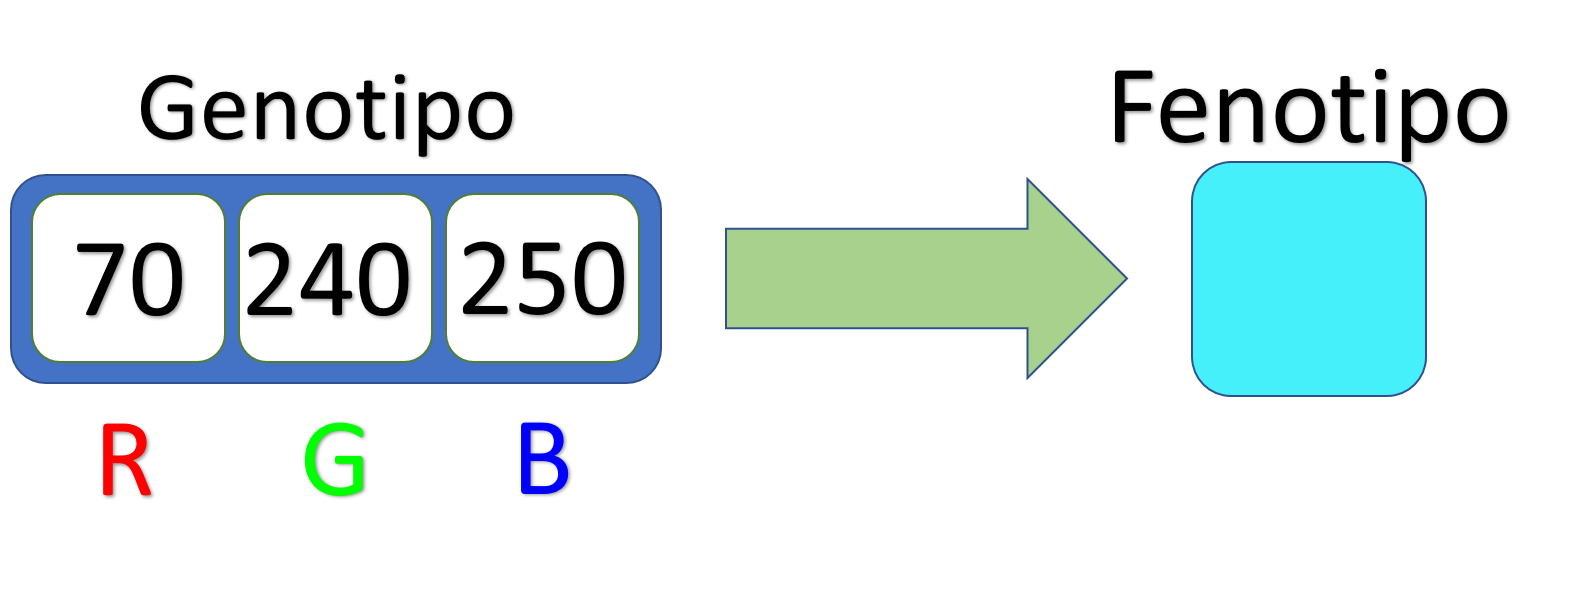
\includegraphics[height=4.5cm]{genotipo-fenotipo}
\end{figure}

Para la selección, recombinación y transformación de los individuos en el proceso de evolución se utiliza un mecanismo de selección y una serie de operadores genéticos \cite{cervigon09}:

\begin{itemize}
\item \textbf{Mecanismos de Selección}: se encargan  de seleccionar un porcentaje de individuos de entre la población que eventualmente participarán de los procesos de cruce y mutación en esa generación. Hay distintos mecanismos de selección de individuos de los cuales dos de los más comunes son el de Selección por Ruleta y Selección por Torneo. La Selección por Ruleta consiste en dar una probabilidad de selección a cada individuo de la forma
\begin{equation}
p_i = \frac{f(i)}{\sum\limits_{j=1}^n f(i)}
\end{equation}
donde $f(i)$ es el valor \textit{fitness} del individuo $i$. Para cada individuo $i$ se define una puntuación acumulada de la forma
\begin{equation}
q_i = \sum\limits_{j=1}^i p_j
\end{equation}
A continuación se genera un número aleatorio $\alpha \in [0,1]$ y se selecciona el individuo $i$ que cumpla $q_{i-1} < \alpha < q_i$, este proceso se repite hasta seleccionar el porcentaje de individuos deseados. 

La Selección por Torneo consiste en elegir un conjunto de individuos al azar de la población, normalmente 2 ó 3 individuos, y seleccionar el individuo con mejor valor \textit{fitness}, este proceso se repite hasta seleccionar todos los individuos deseados.

\item \textbf{Operadores de Cruce}: Se encargan de cruzar los genotipos de los individuos seleccionados. El cruce se realiza entre dos individuos previamente seleccionados denominados padres que se cruzan y generan dos individuos nuevos denominados hijos. Al igual que los mecanismos de selección, existen muchos operadores  para cruzar los genotipos, pero estos operadores son dependientes de la codificación del genotipo. Si el genotipo es una cadena de enteros (codificación más común) el método de cruce más genérico es el Cruce Monopunto. Consiste en seleccionar aleatoriamente una posición idéntica en ambos genotipos de los padres (punto de corte) y generar dos hijos que conserven el mismo genotipo que su padre hasta la posición escogida y, a continuación, intercambiar la otra parte con la del otro padre.
\begin{figure}[H]
\centering
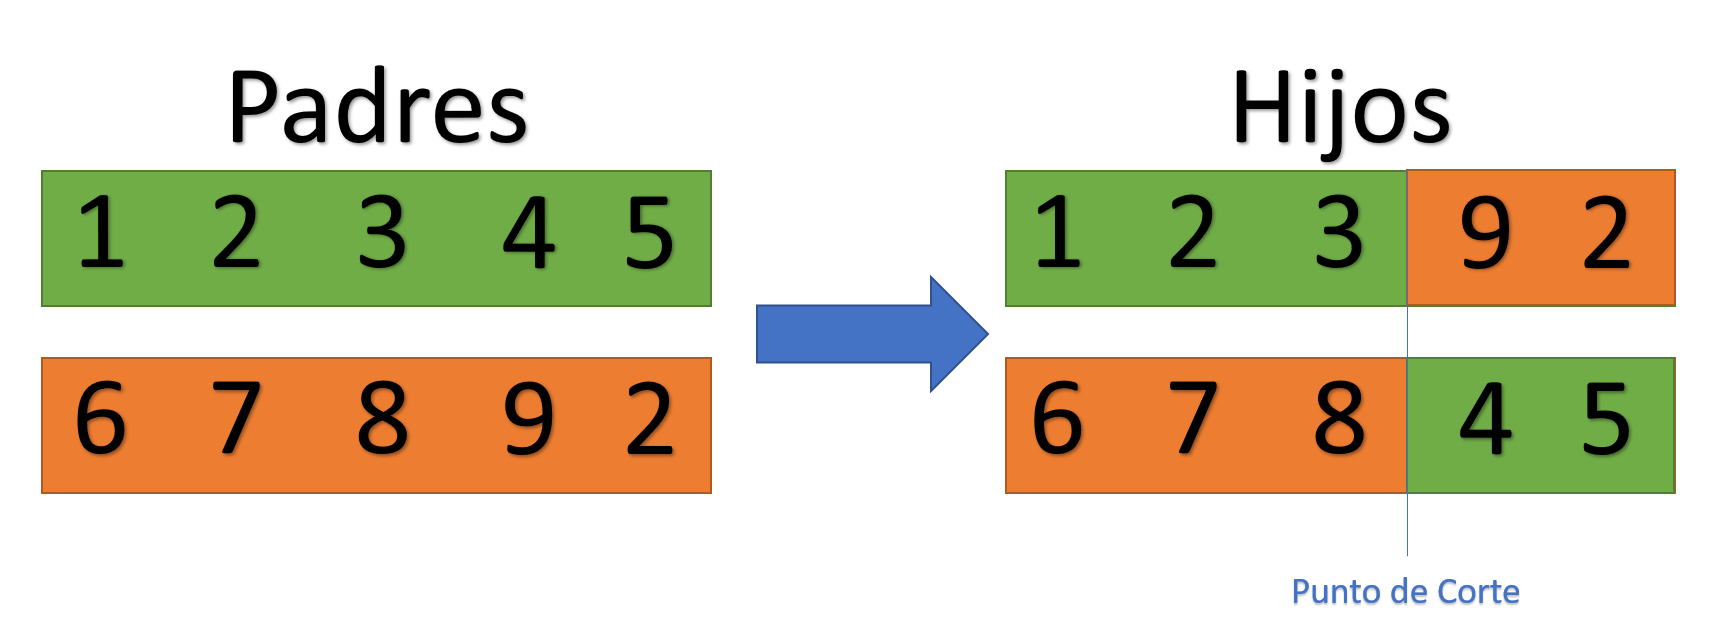
\includegraphics[height=4.5cm]{operador-cruce}
\end{figure}

\item \textbf{Operadores de Mutación}: Estos operadores realizan cambios aleatorios en los valores del genotipo. Hay una gran variedad de operadores de mutación distintos y su posible uso, al igual que con los operadores de cruce, depende de la codificación del genotipo. En una representación del genotipo en forma de cadena de enteros el operador de mutación más utilizado es el Operador de Mutación Aleatorio bit a bit (\textit{Integer Flip Mutation}) el cual recorre toda la cadena del genotipo y cambia un bit (o número) del genotipo por otro aleatorio dependiendo de una probabilidad.
\end{itemize}

Se pueden encontrar una gran variedad de algoritmos evolutivos, siendo algunos más recomendables que otros a la hora de abordar el problema que se quiere resolver o los resultados a obtener. Destacamos los siguientes:
\begin{itemize}
\item \textbf{Algoritmos Genéticos}: Los más comúnmente usados. En ellos el genotipo de los individuos es una cadena de números que posteriormente es decodificada para generar el fenotipo \cite{cervigon09}. Estos algoritmos usan los métodos de selección y operadores de cruce y mutación previamente explicados. 

\item \textbf{Programación Genética}: Se hacen evolucionar programas informáticos con el objetivo de encontrar el más óptimo para una tarea a realizar. La codificación de los programas en el genotipo es realizada mediante árboles en donde cada nodo representa un token del lenguaje de programación escogido. Se explicarán con más detalle en la siguiente sección.

\item \textbf{Evolución Gramatical}: Similar a la programación genética pero usando cadenas de enteros como genotipo que dictan cómo se genera el código informático a través de una Gramática Independiente del Contexto. Se explicará con más detalle posteriormente.
\end{itemize}

\section{Programación genética}
El objetivo de los algoritmos de programación genética es evolucionar programas informáticos escritos en un lenguaje determinado con el fin de encontrar el mejor programa que realice o resuelva un objetivo. En la programación genética el genotipo de los individuos es un árbol formado por nodos. Dependiendo de su contenido los nodos son nodos terminales (expresiones que no pueden ser expandidas, como números o variables) o nodos internos (normalmente representan funciones y contienen nodos hijos, por ejemplo un nodo interno que represente la suma entre dos números el cual tendrá dos nodos hijo donde la información obtenida de cada uno será un número). El fenotipo es el programa final que será ejecutado para evaluar al individuo y la forma de ser generado a partir del genotipo varía dependiendo del lenguaje en el que estén escritos los programas siendo algunos más complejos que otros. En algunos casos el fenotipo es igual al recorrido en inorden del árbol (genotipo) o en otros se necesitará realizar operaciones más complejas para generar el fenotipo \cite{cervigon09}.
\begin{figure}[H]
\centering
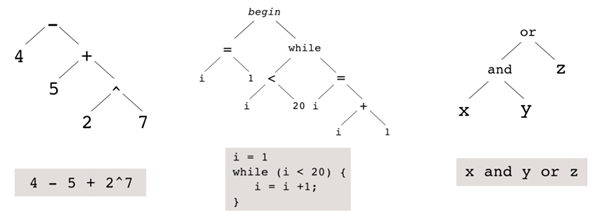
\includegraphics[height=5cm]{genotipo-fenotipo-ejemplo}
\caption{Genotipo y fenotipo de distintos individuos \cite{colmenarApuntes}.}
\end{figure}

Existen distintos métodos para generar los individuos aleatorios de la población inicial:
\begin{itemize}
\item \textit{Grow}: Se va eligiendo aleatoriamente nodos internos o nodos terminales, si se escoge un nodo terminal para una rama del árbol dicha rama se cierra y se prosigue con el resto de ramas abiertas. Si se elige un nodo interno se abren tantas ramas como indique el tipo de nodo y se expanden recursivamente siguiendo el mismo método hasta que todas las ramas hayan sido cerradas. Este método produce una población con árboles de profundidades irregulares.

\item \textit{Full}: Se establece una profundidad máxima del árbol y se van generando nodos internos hasta que se alcanza la profundidad máxima momento en el que se elige únicamente nodos terminales hasta cerrar todas las ramas. Mediante este método la población generada se compone en su totalidad de individuos con árboles completos.

\item \textit{Ramped half-and-half}: Método que usa ambos métodos anteriores, parte de la población es generada usando el método \textit{Full} y la parte restante mediante el método \textit{Grow}. El resultado es una mezcla de árboles irregulares de diferentes profundidades creadas por el método \textit{Grow} y árboles más regulares creados por el método \textit{Full}.
\end{itemize}

Los métodos de selección son los mismo que los usados en los Algoritmos Genéticos como selección por Torneo o Ruleta.
Como la codificación del genotipo ya no es una cadena de valores, los operadores de cruce y mutación comúnmente usados en los algoritmos genéticos (como el cruce monopunto) no pueden usarse y se emplean otros más específicos.

\blankline

El operador de cruce más usado en programación genética, denominado cruce de subárboles, consiste en elegir aleatoriamente en cada padre un punto de cruce (un nodo) y el subárbol que forma es intercambiado con el subárbol del otro padre.

\begin{figure}[H]
\centering
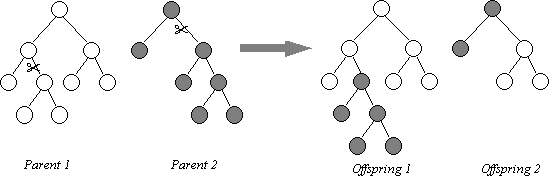
\includegraphics[height=5cm]{cruce-subarboles}
\caption{Operador de cruce de subárboles \cite{tsang2000eddie}.}
\end{figure}

Existen distintos operadores de mutación para árboles, los más comunes son los siguientes:
\begin{itemize}
\item Mutación de subárbol: Solo se aplica una vez por individuo. Selecciona un nodo aleatorio y sustituye todo su subárbol por uno nuevo generado aleatoriamente usando uno de los métodos nombrados anteriormente como \textit{Ramped half-and-half}.

\item Mutación puntual: Elige un nodo aleatorio que cambia por otro nodo generado aleatoriamente (esto puede provocar cambios y conflictos en los subárboles del nodo mutado que han de ser arreglados).

\item Mutación terminal: Un nodo terminal aleatorio se cambia por otro nodo terminal generado aleatoriamente.

\item Mutación de función: Se selecciona un nodo interno de forma aleatoria y se cambia por otro nodo interno generado aleatoriamente pero que preserve las características del nodo anterior (mismo número de nodos hijo, función que devuelva un valor del mismo tipo, etc.).
\end{itemize}

La programación genética no está exenta de problemas y uno muy común es el \textit{Bloating}. Al realizar la operación de cruce, el árbol de los nuevos individuos generados pueden tener un tamaño excesivamente grande y que puede ir a más dado que este puede ser cruzado en generaciones posteriores (llegando a tener individuos con árboles extremadamente largos esparcidos por la población). Además, esto genera la aparición de intrones, grupos de nodos en el genotipo que generan trozos de código que no aportan nada a la funcionalidad del código generado y que intensifican la formación de \textit{Bloating}.

\begin{figure}[H]
\begin{lstlisting}[frame=single, breaklines=no, basicstyle=\fontsize{10}{11}\ttfamily]
    ...
    if (distFantasmaMasCercano > 20) { 
        if (distFantasmaMasCercano < 10) {
            //Sección de programa que nunca llegará a ejecutarse
        }
    }
    ...
\end{lstlisting}
	\caption{Ejemplo de intrón.}
\end{figure}

Hay varios métodos para intentar solventar el problema del \textit{Bloating}:
\begin{itemize}
\item \textit{Naive}: se empeora el fitness precalculado de todos los individuos en la siguiente cantidad
\begin{equation}
\textrm{Valor de empeoramiento del fitness} = k_{empeoramiento} * \textrm{tamano del árbol}
\end{equation}
donde $k_{empeoramiento}$ es una constante previamente elegida. De este modo, los individuos con valores de \textit{fitness} similares pero con un genotipo más largo son penalizados frente a los individuos con genotipos más cortos.

\item \textit{Tarpeian}: trata de eliminar individuos que excedan la extensión media de la población en base a una probabilidad. Si un individuo con longitud de genotipo superior a la media ha sido elegido para su eliminación se le asigna el valor del peor \textit{fitness} posible de tal forma que en la siguiente generación este individuo tenga muy pocas probabilidades de ser seleccionado y se elimine.

\item \textit{Covariant Parsimony Pressure:} \cite{poli2008covariant} Funciona igual que el metodo \textit{Naive} pero empleando un valor de $k_{empeoramiento}$ calculado en cada generación mediante una fórmula que tiene en cuenta características de los genotipos de la población, como su longitud media.
\end{itemize}

La programación genética ya ha sido utilizada para la evolución de un controlador del famoso juego Pac-Man. Koza \cite{koza1992genetic} utilizó la programación genética para evolucionar el código del controlador del personaje principal de Pac-Man de una versión personalizada del juego. Para ello empleó dos tipos de operadores, operadores de alto nivel para la obtención de información del juego (\textit{Distance-to-Pill},
\textit{If-Less-Than-or-Equal}) y operadores de acción (\textit{Advance-to-Food}). Con estos operadores el algoritmo construye y evoluciona el genotipo de los individuos guiándose por la función de fitness, que es básicamente el número total de puntos obtenidos por el Pac-Man antes de morir (obteniendo el fenotipo del individuo y ejecutandolo en el juego). Koza obtuvo resultados muy prometedores con este método.

Alhejali y Lucas \cite{alhejali2010evolving} realizan una implementación muy parecida a la de Koza pero usando operadores de un nivel más alto y abstracto (\textit{isInDanger()}, \textit{toSafety()}, ...) aunque obtuvieron resultados bastante similares. Sin embargo, Brandstetter y Ahmadi \cite{brandstetter2012reactive} obtan por el uso de operadores de acción de bajo nivel (\textit{Up, Down, Left, Right}), obteniendo muy buenos resultados y realizando una comparativa con otros controladores evolucionados mediante programación genética (incluyendo los previamente nombrados). En la comparativa se aprecian mejores resultados con los operadores de bajo nivel que con los operadores de alto nivel o más abstractos.

\section{Gramáticas independientes del contexto}
Una Gramática Independiente del Contexto (en adelante GIC o gramática) es una cuaterna formada por un conjunto de símbolos no terminales, un conjunto de símbolos terminales, un conjunto de reglas de producción (también denominadas expresiones) y un símbolo inicial. Mediante estos símbolos y reglas la Gramática es capaz de generar un Lenguaje Independiente del Contexto\cite{hopcroft_motwani_ullman_2007}\cite{HolgerApuntes}.

\textit{Backus-Naur Form} (BNF) es una notación formal para representar Gramáticas Independientes del Contexto la cual es fácilmente interpretable por el ser humano. Una BNF se compone de Símbolos terminales y no terminales (escritos entre \texttt{< >}). Estos Símbolos no terminales pueden ser expandidos por una serie de expresiones las cuales a su vez contienen un conjunto de Símbolos no terminales o un Terminal. La mayoría de lenguajes informáticos, por ejemplo, tienen una representación escrita en formato BNF \cite{garshol2003bnf}.

\begin{figure}[H]
\centering
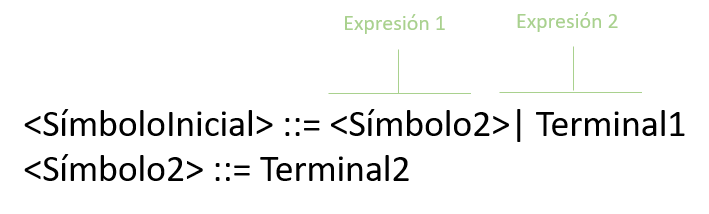
\includegraphics[height=4cm]{bnf}
\end{figure}

Para obtener una derivación (una secuencia de caracteres perteneciente al lenguaje que representa la BNF) se parte del Símbolo Inicial. A partir de aquí se repite recursivamente el siguiente proceso: se procesan, en orden de aparición, todos los símbolos no terminales contenidos en la regla elegida. Para cada símbolo no terminal sin procesar se realiza el mismo proceso, se elige una producción perteneciente al mismo y se vuelve a realizar este proceso de forma recursiva hasta elegir una producción que contenga un terminal, momento en el que el símbolo se da por procesado y se pasa a procesar el siguiente símbolo no terminal sin haber sido completamente procesado. El proceso termina cuando todos los símbolos no terminales han sido procesados.

\begin{figure}[H]
\centering
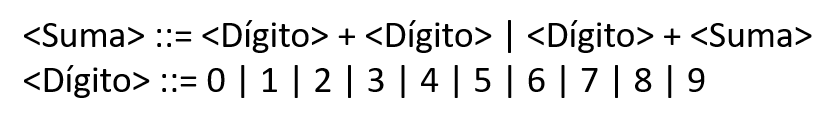
\includegraphics[height=2.2cm]{bnf-ejemplo}
\caption{BNF que representa sumas de dígitos.}
\end{figure}

Para procesar y utilizar una BNF se usa un lector de BNFs que recorre y extrae información de la misma, como los símbolos y terminales que la componen.

\section{Evolución gramatical}
Evolución gramatical (\textit{Grammatical Evolution} en inglés) es un tipo de algoritmo evolutivo basado en la programación genética que permite generar automáticamente expresiones o programas  con el objetivo de encontrar el óptimo que realice una acción o resuelva un problema. A diferencia de la programación genética, donde se utiliza un árbol para codificar el genotipo, en la evolución gramatical se usa un array de enteros como genotipo y una Gramática Independiente del Contexto en notación \textit{Backus-Naur Form} (BNF) para la generación del fenotipo. Estos números enteros que componen el array del genotipo se denominan \textit{codones} y dictan qué producción perteneciente a una regla de la gramática se escoge a la hora de generar el fenotipo. Un ejemplo de genotipo formado por 5 codones tendría la forma: 37, 12, 5, 42, 1. El rango de valores que pueden tomar los codones se determina de antemano.

Para determinar la producción a procesar del símbolo no terminal siendo expandido se utiliza la siguiente fórmula:
\begin{equation}
\textrm{Expresión a escoger} = \textrm{codón} \bmod \textrm{(nº de expresiones para el símbolo a derivar)}
\end{equation}
donde $\bmod$ es la función de módulo entero. Esta fórmula devuelve un número que es la posición de la producción a seleccionar del símbolo no terminal que está siendo expandido \cite{o2012grammatical}.

\begin{figure}[H]
\centering
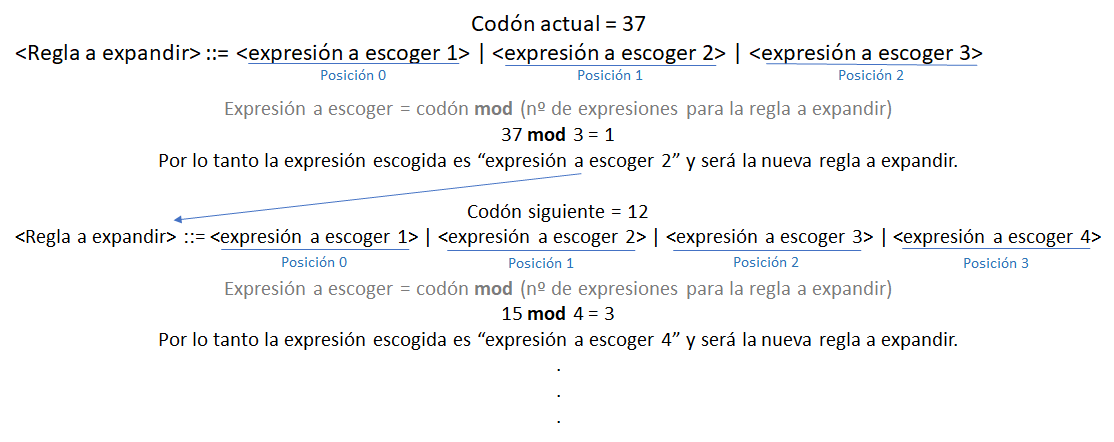
\includegraphics[width=\textwidth]{expandir-codon}
\caption{Ejemplo del proceso que se realizaría para transformar el genotipo mostrado anteriormente al fenotipo que representa.}
\end{figure}

Esta fórmula se aplica en orden a los símbolos no terminales hasta que todos hayan sido procesados, es decir, se hayan alcanzado en todos un símbolo no terminal. A veces esto no se consigue con un único recorrido del genotipo, por lo que se realiza lo que se conoce como \textit{wrapping}, que consiste en  volver a empezar a leer el genotipo desde el principio y seguir expandiendo las reglas todavía sin expandir. El número de veces que se permite realizar \textit{wrapping} por individuo se determina de antemano y si, tras realizar \textit{wrapping} este número de veces no se ha conseguido derivar todos los símbolos, el individuo es descartado.

\begin{figure}[H]
\centering
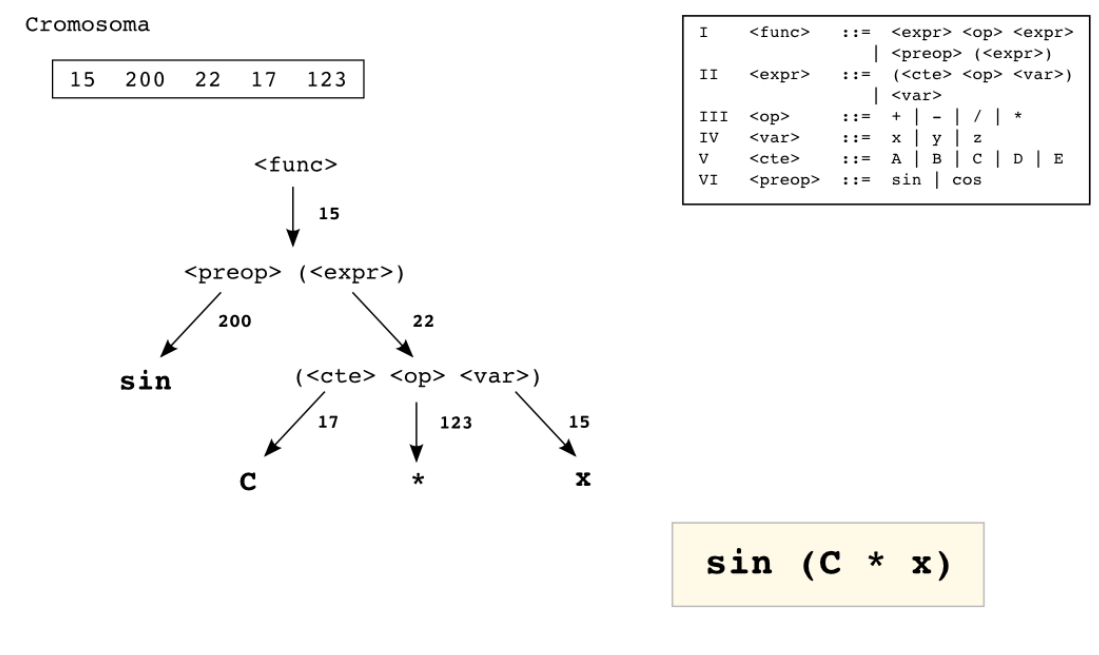
\includegraphics[width=\textwidth]{codon-a-arbol}
\caption{Conversión de un genotipo (cromosoma) a su fenotipo a través del método descrito anteriormente y utilizando la gramática dada \cite{colmenarApuntes}.}
\end{figure}

La estructura de partida de las también llamadas gramáticas evolutivas es muy similar a la de los Algoritmos Genéticos comunes.
\begin{enumerate}
\item Generar una población aleatoria.
\item Evaluar la población usando una función de fitness.
\item Cruzar la población mediante el operador de cruce elegido.
\item Mutar la población mediante el operador de mutación elegido.
\item Repetir desde el punto dos hasta que se alcance el número de generaciones.
\end{enumerate}

Sin embargo, el uso de operadores clásicos de cruce y mutación produce resultados poco óptimos debido a que genera poblaciones muy caóticas, un pequeño cambio en un codón del genotipo puede producir un programa completamente diferente y sin relación con el anterior dificultando en gran medida la convergencia de la población hacia el óptimo. Es por esta razón por la cual distintos operadores se han diseñado específicamente para su uso en gramáticas evolutivas.

La mayoría de las investigaciones se centran en los métodos de cruce debido a que son bastante destructivos (el fenotipo del hijo de dos padres suelen no tener ninguna relación con el fenotipo de sus padres lo que dificulta una evolución convergente). No es fácil dar con un nuevo método que mejore o no empeore el cruce monopunto, como es el caso del cruce homogéneo \cite{O'neill:2003:CGE:608284.608289}, pero hay algunos operadores de cruce que sí mejoran considerablemente el cruce monopunto e intentan minimizar el comportamiento destructivo que tiene el cruce en los algoritmos genéticos, como es el caso de \textit{LHS replacement crossover} \cite{harper2005structure}.

Este operador de cruce trata de cruzar dos individuos moviendo producciones enteras y no secuencias de codones arbitrarias. Para ello selecciona un codón aleatorio del genotipo y busca el símbolo que ha de ser expandido por ese codón a la hora de generar el fenotipo. Desde ese codón se cogen tantos codones como sea necesario para expandir completamente el símbolo (llegar a un símbolo terminal). Es este conjunto de codones el que es insertado en el genotipo del otro individuo y viceversa. Este proceso se puede ver como un ``cortar-pegar'' de trozos del fenotipo de un individuo en el fenotipo del otro individuo obteniendo hijos que poseen un fenotipo relacionado al del padre.

Los operadores de mutación pueden afectar de manera notable al fenotipo del individuo si se muta un codón que expande un símbolo no terminal. Así mismo puede generar mutaciones sin efecto si se genera un nuevo codón que tenga el mismo módulo que el anterior. Se suelen utilizar los operadores de mutación clásicos. Aún así, nuevos operadores de mutación han sido diseñados centrándose en gramáticas evolutivas, como por ejemplo la Mutación Neutral \cite{Oesch2015}. Este operador pretender dar mayor diversidad a la población, para ello muta aleatoriamente codones dándoles un nuevo valor que produzca el mismo módulo que el anterior al generar el fenotipo. Este cambio no afecta directamente al fenotipo (se mantiene igual) pero en las siguientes generaciones en las que el genotipo puede haber cambiado esta mutación neutral si puede tener efecto. Se puede utilizar en conjunto con otro operador de mutación que sí produzca cambios en el fenotipo, por ejemplo la mutación bit a bit.

Además de los operadores también se pueden encontrar cambios en la codificación del genotipo \cite{lourencco2016unveiling} o adaptaciones de distintos tipos de algoritmos genéticos a algoritmos de evolución gramatical con el fin de hacer esta misma más eficiente y efectiva, como es el caso de la evolución diferencial. La evolución diferencial es un algoritmo genético el cual genera una población auxiliar adicional y realiza el cruce entre elementos de la población auxiliar y la población principal. El operador de mutación en vez de generar cambios aleatorios utiliza individuos de la población y los combina mediante una fórmula matemática creando un nuevo individuo. El uso de este algoritmo aplicado a un genotipo-fenotipo del algoritmo de evolución gramatical da lugar al algoritmo denominado \textit{Evolución Diferencial Gramatical} \cite{o2006grammatical}.

Otro método típicamente usado es el \textit{Grammatical Swarm Evolution} el cual es una mezcla de la evolución gramatical y \textit{Particle Swarm Optimization} (Optimización por enjambre de partículas o PSO) \cite{o2004grammatical} \cite{gomez2010particle}. PSO es un algoritmo que intenta explorar todo el espacio de soluciones y así encontrar el máximo/mínimo global y no estancarse en máximos/mínimos locales. Para eso trata la población de individuos como partículas en un ``mapa'' (espacio de soluciones) representadas mediante una ``posición'' (estado actual) que cambia en cada generación dependiendo de la ``velocidad''  de la partícula. Esta ``velocidad'' se calcula en cada generación mediante una fórmula matemática que utiliza distintas variables como la ``posición'' de la mejor partícula actual (óptimo local) en el ``mapa''.

\blankline

Al igual que la programación genética, las gramáticas gvolutivas también han sido usadas previamente para la evolución de controladores de Pac-Man. Galván-López \cite{galvan2010evolving} usó una estrategia similar a la utilizada por Koza (en su implementación mediante programación genética) usando funciones de alto nivel para los operadores de movimiento (\textit{ANG - Avoid Nearest Ghost}) y para los operadores que obtienen información del estado del juego (\textit{avgDistBetGhosts}). Usaron una gramática compuesta por declaraciones \textit{if-else} para la elección del operador de movimiento adecuado basándose en ciertas características del estado actual del juego. Con esta implementación obtuvieron resultado similares a los controladores obtenidos mediante programación genética y con la ventaja que la gramática utilizada se puede cambiar con facilidad (añadiendo o quitando reglas) y obteniendo de este modo distintos comportamientos adaptados a las nuevas funciones disponibles.

Liberatore \cite{Liberatore2014} propuso otra implementación interesante pero esta vez para el controlador de los fantasmas, utilizando gramáticas evolutivas y \textit{Flocking Strategies} para obtener comportamientos y estrategias basados en una inteligencia de colmena.

\section{Algoritmos Evolutivos Multiobjetivo}
Todas las distintas ramas de algoritmos evolutivos que hemos presentado anteriormente comparten la característica de que están enfocados a optimizar  un único objetivo en la  función de \textit{fitness}. Sin embargo, a veces aparecen problemas en los que se buscan soluciones que optimicen más de una variable y se les denomina problemas multiobjetivo.

Si por cada objetivo a optimizar se crea una función fitness para determinar cómo de bueno es el individuo respecto a ese objetivo entonces se busca:
\begin{equation}
Optimizar \{f_i(X) \mid \forall i = 1, \dots, \textrm{nº de objetivos}\}
\end{equation}
donde $f_i$ es la función $i$-ésima de \textit{fitness}.

Por ejemplo, un algoritmo evolutivo que determine dónde invertir en Bolsa podría tener dos objetivos, maximizar las ganancias de la inversión y minimizar el riesgo de pérdidas.

La dificultad de un algoritmo multiobjetivo es determinar el óptimo global, es decir, el individuo que optimiza de la mejor forma todos los objetivos. La solución al ejemplo anterior no es trivial ni única, pues el algoritmo puede dictar una inversión que optimice el beneficio obtenido pero con un alto riesgo de pérdidas así como una inversión segura pero que genera muy pocos beneficios.

\blankline

Se suele emplear la definición de óptimo en un contexto multiobjetivo dada por Vilfredo Pareto, denominado óptimo de Pareto. Se dice que una solución Y domina (es mejor) a otra X si es igual o mejor en todos los objetivos y es estrictamente mejor en al menos un objetivo \cite{cervigon09}.
\begin{figure}[H]
\begin{equation}
f_i(y) \leq f_i(x), (\forall i = 1, \dots, \textrm{nº de objetivos}\}) \wedge \exists f_i(y) < f_j(x)
\end{equation}
\caption{Óptimo de Pareto para un problema de minimización.}
\end{figure}

Normalmente (como en el ejemplo anterior de inversión en bolsa) existen varios óptimos de Pareto, es decir, un conjunto de soluciones que dominan al resto pero que entre ellas no se dominan. A este conjunto de soluciones se le denomina \textit{frente de Pareto}.

\begin{figure}[H]
\centering
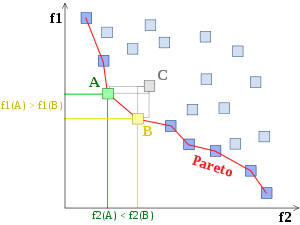
\includegraphics[width=9cm]{pareto}
\caption{Frente de Pareto de un conjunto de soluciones para un problema de minimización. C es una solución dominada por A y B, ambas pertenecientes al frente de Pareto \cite{pictPareto}.}
\end{figure}

A la hora de implementar un algoritmo multiobjetivo podemos elegir entre diferentes  métodos. El más sencillo, y que no altera los esquemas clásicos de los algoritmos evolutivos, es el denominado multiobjetivo mediante Funciones Agregativas que consiste en la creación de una función fitness f como una combinación lineal de funciones en donde cada una representa un objetivo a optimizar.
\begin{equation}
f(x) = \theta_1f_1(x) + \theta_2f_2(x) + \dots + \theta_nf_n(x)
\end{equation}
donde $\theta_i$ son coeficientes utilizados para dar más o menos peso a cada función. El principal problema de este enfoque a problemas multiobjetivo es la dificultad para encontrar los pesos adecuados.

Un método muy utilizado es el desarrollado por Deb, \textit{et al.} denominado NSGA-II (\textit{Non-dominated Sorting Genetic Algorithm}) el cual ofrece buenos resultados pero es bastante exigente computacionalmente, sobretodo para poblaciones grandes \cite{deb2002fast}. El método consiste en la identificación de los distintos frentes de Pareto de la población en la generación actual. Para ello se identifican los individuos pertenecientes al frente de Pareto de la población y se les asigna rango uno, nuevamente se vuelve a identificar el frente de Pareto de la población sin tener en cuenta los individuos que pertenecen al frente de Pareto ya identificado y se les asigna rango dos y se realiza este proceso hasta que todos los individuo de la población tienen asignado un frente de Pareto al que pertenecen. Para los individuos de cada frente de Pareto se calcula una serie de valores denominados \textit{distancias de saturación} respecto a los distintos objetivos. Usando estas distancias de saturación la selección se realiza mediante el método de Torneo, se escogen dos elementos aleatorios de la población y se selecciona el que pertenezca al menor frente de Pareto (rango más bajo). Si ambos individuos pertenecen al mismo frente de Pareto entonces se escoge el que tenga mayor distancia de saturación.

\subsection{JECO}
Como punto de partida para abordar el uso de gramáticas evolutivas hemos decidido emplear el \textit{framework} JECO \cite{jecoGit} (\textit{Java Evolutionary Computation Library}). Inicialmente se valoraron otras opciones como  GEVA \cite{gevaGit}, reutilizar código nuestro o partir de cero.

JECO (Java Evolutionary COmputation) es un framework de inteligencia artificial orientado a la computación evolutiva, creado por José Luis Risco Martín y José Manuel Colmenar Verdugo, con la colaboración posterior de Josué Pagán Ortiz.

Soporta muchas técnicas de programación evolutiva, entre las que nos interesaron las gramáticas evolutivas simples y multiobjetivo (utilizando el algoritmo NSGA-II descrito anteriormente y que utilizaremos en nuestro trabajo), con soporte para el uso de varios hilos de procesamiento.
